\documentclass[times, utf8, zavrsni, numeric]{fer}
\usepackage{booktabs}
\usepackage{listings}
\usepackage{algorithm}
\usepackage{algorithmic}
\usepackage{color}
\usepackage{tikz}
\usepackage{subcaption}
\usepackage{array,multirow,graphicx}

\begin{document}

% TODO: Navedite broj rada.
\thesisnumber{3948}

% TODO: Navedite naslov rada.
\title{Raspoznavanje objekata konvolucijskim neuronskim mrežama}

% TODO: Navedite vaše ime i prezime.
\author{Dario Smolčić}

\maketitle

% Ispis stranice s napomenom o umetanju izvornika rada. Uklonite naredbu \izvornik ako želite izbaciti tu stranicu.

% Dodavanje zahvale ili prazne stranice. Ako ne želite dodati zahvalu, naredbu ostavite radi prazne stranice.
\zahvala{Zahvaljujem doc. dr. sc. Siniši Šegviću na mentorstvu i pomoći pruženoj pri pisanju završnog rada.}

\tableofcontents

\chapter{Uvod}
Računalni vid je područje koje uključuje metode za dohvaćanje, obrađivanje i shvaćanje slika i općenito podataka velikih dimenzija te je zanimljivo područje računalne znanosti zbog mogućnosti široke primjene u današnjem svijetu. Jedna od podgrana ovog područja je raspoznavanje objekata.

Ljudi su sposobni prepoznati mnoštvo različitih objekata s jako malo truda no za računala je to složen proces koji ima brojna ograničenja koja ljudi nemaju. Uzmimo u obzir da se slika u računalu reprezentira kao višedimenzionalni niz jačina svjetlosti. Promjene u prikazu objekta poput različite orijentacije, skaliranja, i osvjetljenja objekta su u digitalnim slikama predstavljene s različitim podatcima. Objekt također može biti i zaklonjen. Dobar model raspoznavanja mora biti otporan na ove varijacije te je zato problem raspoznavanja objekata još uvijek neriješen. U zadnjih nekoliko desetljeća su razvijene brojne metode kojima se pokušava riješiti spomenuti problem.
Za razliku od pisanja klasičnih algoritama poput sortiranja brojeva za problem klasifikacije objekata nije očito kako bi se mogao napisati takav algoritam gdje su sve varijacije ulaza posebno obrađene u kodu. Zato se za klasifikaciju objekata koristi pristup usmjeren na podatke (engl. \textit{data-driven approach}). Programu se da veliki broj ulaza s velikom količinom primjera za svaku klasu te se razvije algoritam učenja koji učitava date primjere te uči o vizualnom prikazu svake klase. Takve programe nazivamo klasifikatorima.

U zadnjih nekoliko desetljeća su razvijeni različiti klasifikatori za što točnije prepoznavanje objekata. Među tim klasifikatorima su i umjetne neuronske mreže. Ispostavilo se da se s dubokim neuronskim mrežama trenutno dobivaju najbolji rezultati za problem klasifikacije. Najkorišteniji oblik dubokih neuronskih mreža u računalnom vidu su konvolucijske neuronske mreže.

Cilj ovog rada je razviti implementaciju konvolucijske neuronske mreže za primjenu na osobnim računalima, optimirati hiperparametre mreže te vrednovati učinak naučene mreže. Razvijena mreža će se testirati na skupu MNIST rukom pisanih znamenki.
\chapter{Neuronske mreže}
Područje umjetnih neuronskih mreža (engl. \textit{Artificial Neural Networks - ANN}) je prvotno bilo inspirirano s modeliranjem biološkog živčanog sustava, a tek kasnije se počelo koristiti u sklopu strojnog učenja. 
\section{Neuron}
Radi razumijevanja neuronske mreže potrebno je prvo razumjeti funkcioniranje jednog neurona. Ljudski živčani sustav se sastoji od otprilike 86 bilijuna neurona koji su povezani sa $10^{14}$ do $10^{15}$ sinapsi. Svaki neuron dobiva svoje ulazne signale kroz dendrite i šalje izlazni signal kroz akson. Akson je sa sinapsama spojen s dendritima drugih neurona. Na slici ~\ref{fig:bio-neuron} možemo vidjeti izgled biološkog neurona.
\begin{figure}
    \centering
    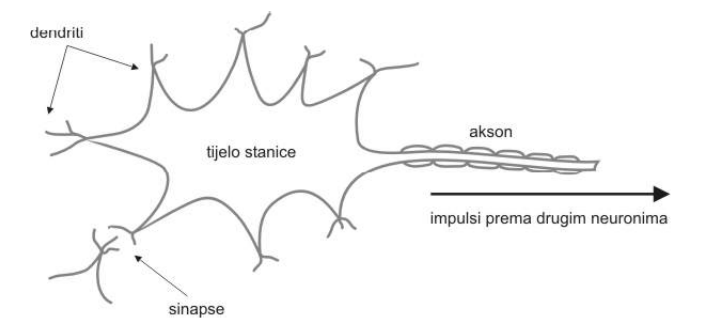
\includegraphics[width=12cm]{img/bio-neuron.png}
    \caption{Biološki neuron}
    \label{fig:bio-neuron}
\end{figure}

U modelu umjetnog neurona signali koji putuju aksonom (npr. \textbf{$x_{0}$}) se množe sa sinaptičkim snagama dendrita(težinama) drugih neurona (npr. \textbf{$w_{0}$}). Ideja je da se sinaptičke snage mogu mijenjati s učenjem te određuju utjecaj jednog neurona na drugi. Svaki neuron ima aktivacijsku funkciju koja uzima sumu umnoška ulaza neurona s pripadnim težinama i praga ($\theta$) te ih preslikava na izlaz neurona koji modelira signal na aksonu($y$). Na slici ~\ref{fig:umj-neuron} možemo vidjeti model umjetnog neurona. 
\begin{figure}
    \centering
    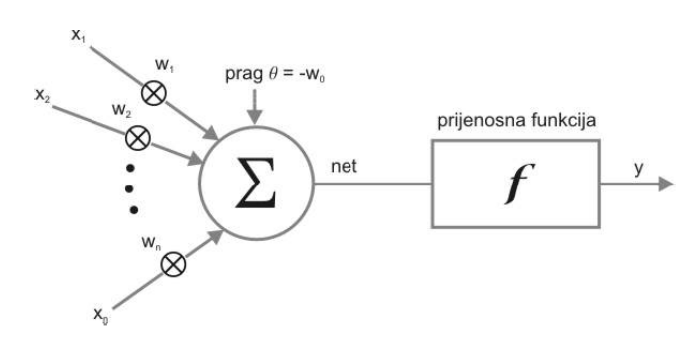
\includegraphics[width=12cm]{img/umj-neuron.png}
    \caption{Umjetni neuron}
    \label{fig:umj-neuron}
\end{figure}

Neka su ulazi označeni sa $x_{1},x_{2},...,x_{n}$ a njihove pripadne težine sa $w_{1},w_{2},...,w_{n}$, i prag sa $\theta$. Onda se izlaz neurona može zapisati kao:
\begin{equation}
y = f(\displaystyle\sum_{i=1}^{n}x_iw_i + \theta)
\end{equation}

Radi pojednostavljenja se često uzima oznaka $w_0$ umjesto $\theta$ te se dodaje jedan ulaz $x_0$ koji je stalno jednak 1. S ovom modifikacijom izlaz neurona se može izraziti kao:
\begin{equation}
y = f(\displaystyle\sum_{i=0}^{n}x_iw_i)
\end{equation}
\subsection{Aktivacijske funkcije}\label{Aktivacijske funkcije}
Postoje veliki izbor aktivacijskih funkcija no u praksi se koriste samo neke koje su se pokazale korisnima. Spomenuti ćemo četiri različite aktivacijske funkcije (slika ~\ref{fig:aktivacijske-funkcije}) te njihove karakteristike.

\begin{figure}
\centering
\begin{subfigure}[b]{0.5\textwidth}
\centering
\begin{tikzpicture}
  \draw[->] (-2,0) -- (2,0) node[right] {$x$};
  \draw[->] (0,-2) -- (0,2) node[above] {$f(x)$};
  \draw[scale=0.5,domain=-3:3,smooth,variable=\x,blue] plot ({\x},{\x});
\end{tikzpicture}
\caption{Linearna funkcija}
\label{fig:linear}
\end{subfigure}%
\begin{subfigure}[b]{0.5\textwidth}
\centering
\begin{tikzpicture}
  \draw[->] (-2,0) -- (2,0) node[right] {$x$};
  \draw[->] (0,-2) -- (0,2) node[above] {$f(x)$};
  \draw[scale=1,domain=-2:2,smooth,variable=\x,blue] plot ({\x},{tanh(\x*3)});
\end{tikzpicture}
\caption{Sigmoidalna funkcija}
\label{fig:sigmoid}
\end{subfigure}%

\begin{subfigure}[b]{0.5\textwidth}
\centering
\begin{tikzpicture}
  \draw[->] (-2,0) -- (2,0) node[right] {$x$};
  \draw[->] (0,-2) -- (0,2) node[above] {$f(x)$};
  \draw[scale=1,domain=-2:0,smooth,variable=\x,blue] plot ({\x},{-1});
  \draw[scale=1,domain=-1:1,smooth,variable=\y,blue] plot ({0},{\y});
  \draw[scale=1,domain=0:2,smooth,variable=\x,blue] plot ({\x},{1});
\end{tikzpicture}
\caption{Funkcija skoka}
\label{fig:step}
\end{subfigure}%
\begin{subfigure}[b]{0.5\textwidth}
\centering
\begin{tikzpicture}
  \draw[->] (-2,0) -- (2,0) node[right] {$x$};
  \draw[->] (0,-2) -- (0,2) node[above] {$f(x)$};
  \draw[scale=1,domain=-2:0,smooth,variable=\x,blue] plot ({\x},{0});
  \draw[scale=1,domain=0:1.5,smooth,variable=\x,blue] plot ({\x},{\x});
\end{tikzpicture}
\caption{Linearna rektifikacijska funkcija}
\label{fig:relu}
\end{subfigure}%
\caption{Različite aktivacijske funkcije}
\label{fig:aktivacijske-funkcije}
\end{figure}

Najobičnija aktivacijska funkcija je linearna aktivacijska funkcija koja je preslikava svoj ulaz pomnožen s nekom konstantom na izlaz. Ovakav tip aktivacijske funkcije se ne koristi u dubokim neuronskim mrežama zato što onemogućava učenje mreže. 

Step funkcije u neuronima funkcioniraju kao prekidači. Izlaz funkcije može poprimiti samo dvije različite vrijednosti ovisno o tome da li je ulaz manji ili veći od nekog praga. Primjer jedne ovakve funkcije je:
\begin{equation}
  f(x) = \begin{cases}
    0, & \text{$x<0$}\\
    1, & \text{$x\geq0$}
  \end{cases}
\end{equation}
Ovakva funkcija je korisna za binarne klasifikatore ali se ne koristi u dubokim neuronskim mrežama. Jedan od razloga je to što je za algoritam unazadne propagacije (kasnije objašnjen) potrebna derivabilna ili po dijelovima derivabilna funkcija. Također zbog same definicije funkcije mala promjena ulaza može dovesti do potpuno suprotne aktivacije neurona čak iako su ulazi jako slični što je nepoželjno svojstvo za našu primjenu.

Sigmoidalne aktivacijske funkcije se najčešće koriste u praksi kod dubokih neuronskih mreža. Ovakve funkcije su derivabilne na cijeloj domeni i ograničene su što su dobra svojstva za algoritam unazadne propagacije i učenje mreže. Dvije najčešće korištene sigmoidalne funkcije su logistička funkcija i funkcija hiperbolnog tangensa. Primjer logističke funkcije dan je u izrazu ~\ref{eq:logistic}. 
\begin{equation}\label{eq:logistic}
f(x) = \frac{1}{1-e^{-kx}}
\end{equation}
U ovom radu se neće koristiti logistička funkcija već funkcija hiperbolnog tangensa koja se pokazala boljom u praksi \citep{lecun1998gradient}. Po uzoru na \citep{lecun1998gradient} koristit će se skalirana funkcija hiperbolnog tangensa prema izrazu ~\ref{eq:htan} čija je derivacija dana sa ~\ref{eq:htan-der}
\begin{equation}\label{eq:htan}
f(x) = 1.7159\tanh\left(\frac{2}{3}x\right)
\end{equation}
\begin{equation}\label{eq:htan-der}
\dfrac{f(x)}{dx} = 1.444\left(1-\tanh^2\left(\frac{2}{3}x\right)\right)
\end{equation}

Još jedna aktivacijska funkcija koja je u zadnje vrijeme davala jako dobre rezultate je linearna rektifikacijska funkcija definirana kao:
\begin{equation}\label{eq:relu}
f(x) = max(0, x)
\end{equation}
Prema \citep{krizhevsky2012imagenet} korištenjem ove aktivacijske funkcije je postignuta čak 6 puta brža konvergencija mreže. Funkcija je po dijelovima derivabilna i nije linearna te je također vrlo jeftina za izračunat (dovoljan je jedan uvjet grananja u kodu).

\section{Arhitektura neuronske mreže}
Povezivanjem velikog broja neurona nastaju neuronske mreže. Neuronske mreže su modelirane kao kolekcije neurona koje su povezane acikličkim grafom. Neuroni u neuronskim mrežama su najčešće organizirani po slojevima (slika ~\ref{fig:neuronska-mreza}). Razlikujemo ulazni, izlazni i skriveni sloj. U ulaznom sloju se na ulaze neurona dovode podatci koje je potrebno klasificirati. Na primjer, za rukom pisane znamenke bi pojedini ulaz bio pisana znamenka. Izlazi neurona ulaznog sloja su spojeni s ulazima neurona skrivenog sloja. Skrivenih slojeva može biti više pa su zato izlazi neurona skrivenih slojeva povezani s ulazima neurona idućih skrivenih slojeva ili s ulazima neurona izlaznog sloja. Izlaz iz neurona izlaznog sloja se interpretira kao klasa koju je mreža klasificirala. Na primjer, ako se klasificiraju rukom pisane znamenke onda postoji 10 različitih klasa i deset neurona u izlaznom sloju. Na temelju tog izlaza (najčešće u obliku brojeva od 0 do 1) se inerpretira rezultat klasifikacije neuronske mreže. Slojevi su najčešće potpuno povezani poput primjera na slici ~\ref{fig:neuronska-mreza}. To znači da su svi neuroni trenutnog sloja povezani sa svim neuronima sljedećeg sloja.

\begin{figure}
    \centering
    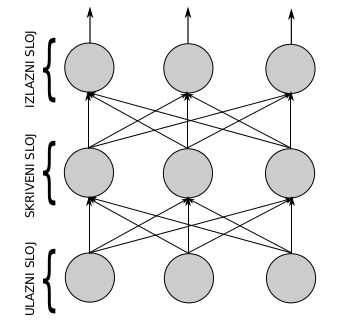
\includegraphics[width=8cm]{img/slojevi-neuronska-mreza.png}
    \caption{Potpuno povezana neuronska mreža sa jednim skrivenim slojem}
    \label{fig:neuronska-mreza}
\end{figure}

Dubokim neuronskim mrežama nazivamo mreže koje imaju dva ili više skrivenih slojeva. Ispostavilo se da su duboke neuronske mreže pogodnije za kompleksnije probleme klasifikacije i da ostvaruju dobre rezultate. Možemo reći da svaki sloj mreže obrađuje podatke na drugoj razini apstrakcije i na temelju tih podataka donosi neku odluku, odnosno daje neki izlaz. Kretanjem od ulaznog sloja prema izlaznom razina apstrakcije se povećava te se grade kompleksniji i apstraktniji koncepti odlučivanja. Ulazni sloj obrađuje podatke na razinama piksela dok izlazni sloj radi na najapstraktnijoj razini i daje rezultat klasifikacije. Intuitivno bismo mogli reći da s većim brojem slojeva možemo preciznije dekomponirati apstraktni problem klasifikacije na niz jednostavnih odluka koje se mogu donijeti na razinama piksela. S većim brojem slojeva je ta dekompozicija finija i preciznija.

Ono što u stvarnosti duboke neuronske mreže rade je simuliranje nelinearne funkcije s velikim brojem parametara. Kada je mreža "naučena", funkcija koju ona simulira je točno ta funkcija koja za dane ulaze daje takve izlaze koji se interpretiraju kao točni rezultati klasifikacije. Intuitivno je jasno da su za probleme klasifikacije često potrebne složene funkcije koje nisu jednostavne. Veći broj slojeva duboke neuronske mreže povećava tu složenost i omogućuje pronalazak takvih funkcija.

\section{Učenje neuronskih mreža}
Pošto neuronske mreže imaju milijune parametara (težina) koje je potrebno odrediti kako bi mreža radila dobru klasifikaciju potrebno je znati kako odrediti te parametre. Dva algoritma su ključna za rad neuronske mreže i za njezino učenje a to su: algoritam \textit{feedforward} i algoritam sa širenjem pogreške unatrag (engl. \textit{backpropagation}).

\subsection{Algoritam feedforward}
Algoritam feedforward omogućava rad neuronske mreže. Algoritam je vrlo jednostavan. Za svaki sloj se  računa njegov izlaz krećući od ulaznog. Ulaz ulaznog sloja su podatci za klasifikaciju dok je njegov izlaz ulaz sljedećeg sloja. Jedino na što treba obratiti pažnju je povezanost slojeva koja za svaki neuron određuje njegovu povezanost s neuronima prethodnog sloja. Algoritam je opisan sa pseudokodom ~\ref{alg:feedforward}.

\renewcommand{\algorithmicfor}{\textbf{za}}
\renewcommand{\algorithmicend}{\textbf{kraj}}
\renewcommand{\algorithmicwhile}{\textbf{dok}}
\renewcommand{\algorithmicdo}{\textbf{radi}}
\renewcommand{\algorithmicif}{\textbf{ako}}
\renewcommand{\algorithmicelse}{\textbf{inače}}
\renewcommand{\algorithmicthen}{\textbf{onda}}
\floatname{algorithm}{Pseudokod}
\begin{algorithm}
\caption{Feedforward}
\label{alg:feedforward}
\begin{algorithmic}
\STATE \textbf{Ulaz:} $x$
\FOR{svaki sloj od ulaznog do izlaznog}
\STATE{Izračunaj izlaz sloja za ulaz $x$}
\STATE{$x \leftarrow$ izlaz trenutnog sloja}
\ENDFOR
\end{algorithmic}
\end{algorithm}
\subsection{Algoritam backpropagation}
Neuronsku mrežu se može shvatiti kao funkciju više varijabli. Varijable su težine na prijelazima neurona a izlaz iz funkcije je pogreška mreže. U promatranju te funkcije smatramo da je ulaz konstantan i da nije varijabla. Cilj je minimizirati pogrešku mreže što se svodi na pretraživanje \textit{n}-dimenzionalnog prostora gdje je \textit{n} ukupan broj težina u mreži. Pogreška u takvom prostoru se može vizualizirati kao hiper-površina sa više lokalnih minimuma.

Ideja algoritma backpropagation je određivanje greške i gradijenata u svakom sloju te ažuriranje težina na temelju gradijenata tako smanjujući grešku neuronske mreže (gradijentni spust). Prvo se pomoću algoritma feedforward dobije odziv mreže za neki ulaz. Zatim se izračunaju greške izlaznog sloja (greške se računaju na svakom neuronu). Zatim se za prethodni sloj određuje utjecaj neurona na greške u idućem sloju te se izračuna greška prethodnog sloja. Zatim se izračuna gradijent greške po težinama koje povezuju te slojeve te se težine ažuriraju. Ovaj postupak se ponavlja za svaki ulaz i određen broj puta.

U svim oznakama koje slijede vrijedi konvencija označavanja trenutnog sloja sa \textit{j} te prethodnog sloja sa \textit{i}, izlaza neurona sa \textit{y} te ukupan ulaz neurona sa \textit{z}. Stoga $y_{i}$ označava izlaz \textit{i}-tog neurona prethodnog sloja a $y_{j}$ izlaz \textit{j}-tog neurona trenutnog sloja, $z_{j}$ ulaz \textit{j}-tog neurona trenutnog sloja, $b_j$ prag j-tog neurona trenutnog sloja te $w_{ij}$ težinu koja spaja i-ti neuron prethodnog sloja sa j-tim neuronom trenutnog sloja.

Da bi se odredila grešku izlaznog sloja potrebno je prvo odrediti funkciju pogreške. Najčešće se koristi srednja kvadratna pogreška:
\begin{equation}\label{eq:sr-kv-pogr}
  E = \frac{1}{2}\sum_j(t_j-y_j)^2
\end{equation}

Parametar $t_j$ predstavlja očekivani izlaz j-tog neurona. Greška trenutnog sloja se definira kao:
\begin{equation}\label{eq:error}
\dfrac{\partial E}{\partial z_j} = \dfrac{\partial E}{\partial y_j} \dfrac{\partial y_j}{\partial z_j}
\end{equation}

Parcijalna derivacija pogreške po izlazu neurona $y_j$ za srednju kvadratnu pogrešku se može raspisati kao:
\begin{equation}\label{eq:sr-kv-pogr-der}
\dfrac{\partial E}{\partial y_j} = \frac{1}{2}\dfrac{\partial}{\partial y_j}(t_j-y_j)^2 = -(t_j - y_j)
\end{equation}

Druga parcijalna derivacija u izrazu ~\ref{eq:error} je jednaka derivaciji aktivacijske funkcije. Derivacija aktivacijske funkcije skaliranog hiperbolnog tangensa je već dana u izrazu ~\ref{eq:htan-der}.

Nakon računanja greške trenutnog sloja računa se greška prethodnog sloja koja je dana s izrazom:
\begin{equation}\label{eq:error-prethodni}
\dfrac{\partial E}{\partial z_i} = \dfrac{\partial E}{\partial y_i} \dfrac{\partial y_i}{\partial z_i} 
\end{equation}

Druga parcijalna derivacije je ponovno jednaka derivaciji aktivacijske funkcije a parcijalna derivacija pogreške po izlazu neurona prethodnog sloja se dobije sumiranjem utjecaja neurona na sve neurone trenutnog sloja:
\begin{equation}\label{eq:dE/yi}
\dfrac{\partial E}{\partial y_i} = \sum_j\dfrac{\partial E}{\partial z_j}\dfrac{\partial z_j}{\partial y_i} 
\end{equation}

Raspišimo $z_j$ kao:
\begin{equation}\label{eq:ulaz-neruona}
z_j = \sum_i w_{ij}y_i + b_j
\end{equation}

Uvrštavanjem ~\ref{eq:ulaz-neruona} u ~\ref{eq:dE/yi} se dobiva sljedeći izraz:
\begin{equation}\label{eq:dE/yi2}
\dfrac{\partial E}{\partial y_i} = \sum_j\dfrac{\partial E}{\partial z_j}\dfrac{\partial z_j}{\partial y_i} = \sum_j w_{ij}\dfrac{\partial E}{\partial z_j}
\end{equation}

Na kraju se određuju parcijalne derivacije po težinama i pragovima:
\begin{equation}\label{eq:der-w}
\dfrac{\partial E}{\partial w_{ij}} = \dfrac{\partial E}{\partial z_j}\dfrac{\partial z_j}{\partial w_{ij}} = \dfrac{\partial E}{\partial z_j}y_i
\end{equation}
\begin{equation}\label{eq:der-b}
\dfrac{\partial E}{\partial b_j} = \dfrac{\partial E}{\partial z_j}\dfrac{\partial z_j}{\partial b_j} = \dfrac{\partial E}{\partial z_j}*1
\end{equation}

Nakon čega se težine i pragovi ažuriraju u ovisnosti o stopi učenja $\eta$:
\begin{equation}\label{eq:azuriraj-w}
w_{ij} \leftarrow w_{ij} - \eta\dfrac{\partial E}{\partial w_{ij}} = w_{ij} - \eta * y_i  \dfrac{\partial E}{\partial z_j}
\end{equation}
\begin{equation}\label{eq:azuriraj-b}
b_{j} \leftarrow b_{j} - \eta\dfrac{\partial E}{\partial b_{j}} = b_{j} - \eta \dfrac{\partial E}{\partial z_j}
\end{equation}

Stopa učenja $\eta$ je mali pozitivni broj koji nam govori koliko brzo ćemo se kretati u smjeru negativnog gradijenta. Gradijent pokazuje u smjeru rasta funkcije pa je zato kod ažuriranja težina i pragova potrebno dodati negativan predznak jer pokušavamo minimizirati funkciju.

\begin{algorithm}
\caption{Backpropagation}
\label{alg:backpropagation}
\begin{algorithmic}
\STATE \textbf{Ulaz:} D (skup za učenje), $\eta$ (stopa učenja)
\STATE{Inicijaliziraj težine na male slučajno generirane vrijednosti}
\WHILE{nije ispunjen uvjet zaustavljanja}
\FOR{svaki (x, t) iz D}
\STATE{Izračunaj izlaz svakog sloja mreže za ulaz x}
\STATE{Izračunaj pogrešku izlaznog sloja prema formulama ~\ref{eq:error} i ~\ref{eq:sr-kv-pogr-der}}
\FOR{svaki sloj od izlaznog do ulaznog}
\STATE{Izračunaj pogrešku prethodnog sloja prema formulama ~\ref{eq:error-prethodni} i ~\ref{eq:dE/yi2}}
\STATE{Izračunaj parcijalne derivacije pogreške po težinama i pragovima prema formulama ~\ref{eq:der-w} i ~\ref{eq:der-b}}
\STATE{Ažuriraj težine i pragove prema formulama ~\ref{eq:azuriraj-w} i ~\ref{eq:azuriraj-b}}
\ENDFOR
\ENDFOR
\ENDWHILE
\end{algorithmic}
\end{algorithm}

Algoritam backpropagation je opisan sa pseudokodom ~\ref{alg:backpropagation}. Uvjet zaustavljanja algoritma je najčešće unaprijed zadan broj iteracija. Jedan prolaz algoritma kroz cijeli skup za učenje nazivamo epohom. Uvjet ne mora nužno biti zadan brojem epoha ili iteracija, također je moguće da se kao uvjet postavi minimalna pogreška izlaza tj, da algoritam staje kad je pogreška dovoljno mala.

Prethodno opisani algoritam koristi stohastički gradijentni spust što znači da se težine ažuriraju nakon svakog ulaza. To znači da nije nužno da se uvijek kreće u smjeru negativnog gradijenta na razini cijelog skupa za učenje. Ovakva varijanta gradijentnog spusta više oscilira te je upravo zbog tog svojstva otpornija na zapinjanje u lokalnim minimumima. Standardna varijanta gradijentnog spusta ažurira težine ili nakon nekog određenog broja ulaza (engl. \textit{batch}) ili nakon svake epohe. U obzir se uzima prosjek gradijenata na svim obrađenim ulazima te je zato ova varijanta stabilnija i ima manje oscilacije ali zato ima veće šanse zapinjanja u lokalnim minimumima te je puno sporija. U ovom radu će se koristiti navedeni stohastički gradijentni spust pošto se u praksi pokazao veoma efikasnim a ujedno je računski puno manje zahtjevan od standardnog.

\chapter{Konvolucijske neuronske mreže}
Konvolucijske neuronske mreže se mogu smatrati proširenjima standardnih neuronskih mreža koje su se pokazale učinkovitijima prilikom klasifikacija slika. Neuroni u konvolucijskim neuronskim mrežama su dvodimenzionalni i nazivamo ih mapama značajki (engl. \textit{feature maps}). Ulaz je također dvodimenzionalan a umjesto težina se koriste jezgre (engl. \textit{kernels}).

\section{Struktura mreže}
Konvolucijske neuronske mreže su građene od tri različite vrste slojeva: konvolucijski slojevi, slojevi sažimanja i potpuno povezani slojevi. Na ulazu mreže se nalazi jedna monokromatska ili višekanalna slika u boji. Zatim slijede naizmjence konvolucijski slojevi i slojevi sažimanja. Mape značajki u tim slojevima u svakom sloju postaju sve manjih dimenzija krećući se od ulaznog sloja. Zadnji takav sloj je dimenzija 1 $\times$ 1. Na takav sloj se vežu potpuno povezani slojevi koji su jednodimenzionalni te se ponašaju kao obične neuronske mreže opisane u prethodnom poglavlju. Primjer ovakve strukture vidimo na slici ~\ref{fig:konvolucijska-mreza}.

\begin{figure}
    \centering
    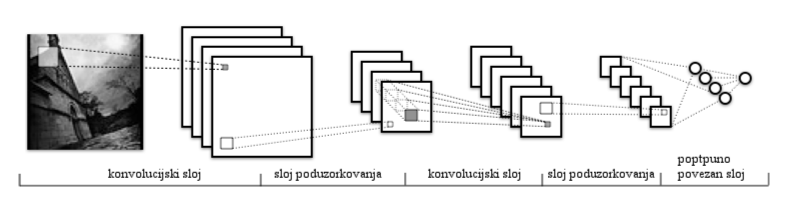
\includegraphics[width=14cm]{img/konvolucijska-mreza.png}
    \caption{Konvolucijska neuronska mreža}
    \label{fig:konvolucijska-mreza}
\end{figure}

\subsection{Konvolucijski slojevi}
Konvolucijski slojevi uzimaju mape na ulazu sloja te rade 2D konvoluciju s jezgrama. Sa $M^j$ su označene dimenzije mapa j-tog sloja, te sa $K^j$ dimenzije jezgri koje povezuju mape prethodnog sloja s mapama trenutnog sloja. Radi jednostavnosti će se koristiti kvadratne mape značajki i kvadratne jezgre te kada se govori o dimenziji $M^j$ misli se na $M^j \times M^j$ (ekvivalentno i s dimenzijama jezgri). Također je sa $S$ označen korak pomaka jezgre po širini i visini prilikom konvolucije. Veličina mapa značajki u nekom sloju dana je s izrazom:
\begin{equation}
M^j = \frac{M^{j-1} - K^j}{S} + 1
\end{equation}

Konvolucija se tvori prolazom kroz ulaznu mapu s prozorom jednake veličine kao i jezgra te se množe vrijednosti ulazne mape unutar prozora sa korespondentnim vrijednostima jezgre (može se zamisliti kao da se preklopi jezgra preko dijela ulazne mape te se množe vrijednosti koje su jedna na drugoj). Sumiraju se dobiveni umnošci za sve ulazne mape značajki i dodaje se prag te se računa izlaz aktivacijske funkcije koji se zapisuje u odgovarajući neuron izlazne mape značajki. Pod pojmom neuron u ovom kontekstu se misli na jednu jedinicu mape značajki. Dakle jedna mapa značajki dimenzije $M^j$ ima $M^j \times M^j$ neurona. Nakon toga se okvir pomiče za $S$ vodoravno, ili okomito ako se nalazi na kraju reda te se cijeli proces ponavlja za sljedeći neuron.

Vidljivo je da na jedan neuron izlazne mape značajki utječu samo dijelovi ulaznih mapi značajki koji su unutar okvira koji je potreban za taj neuron. To područje ulazne mape značajki "vidljivo" neuronu se naziva vizualnim ili receptivnim poljem neurona. Ako se neuron u izlaznoj mapi nalazi na koordinatama $(x, y)$ onda je njegovo vizualno polje definirano s kvadratom dimenzija jednakih dimenzijama jezgre $K^j$, a koordinate gornjeg lijevog kuta vizualnog polja $(x', y')$ u koordinatnom sustavu ulaznih mapi značajki su definirane kao:
\begin{equation}
x' = x*S
\end{equation}
\begin{equation}
y' = y*S
\end{equation}

\begin{figure}
    \centering
    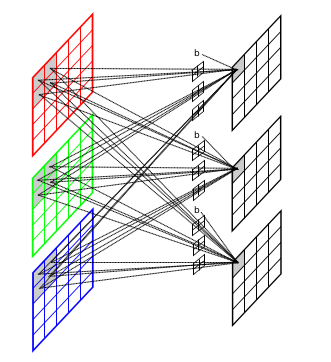
\includegraphics[width=7cm]{img/konvolucija.png}
    \caption{Prvi koraci konvolucija za sve mape značajki}
    \label{fig:konvolucija}
\end{figure}

Neka je $M^j_k$ k-ta mapa j-tog sloja te $w^j_{ik}$ jezgra koja povezuje k-tu mapu j-tog sloja s i-tom mapom prethodnog sloja. Svaka mapa značajki ima po jedan prag $b^j_k$. Pošto su mape značajki i njihove jezgre dvodimenzionalne njihovi elementi su indeksirani sa zagradama. Tako će vrijednost mape značajki na lokaciji $(x, y)$ biti jednaka $M^j_k (x, y)$ a jezgre $w^j_{ik} (x, y)$. Uz ovaj sustav oznaka vrijednost mape k u sloju j na lokaciji $(x, y)$ možemo prikazati sa sljedećim izrazom:
\begin{equation}\label{eq:neuron-conv}
M^j_k (x, y) = f(\sum_i \sum_{x'=0}^{K-1} \sum_{y'=0}^{K-1} M^{j-1}_i (x' + x, y' + y) w^j_{ik} (x', y') + b^j_k )
\end{equation}

Funkcija u jednadžbi je aktivacijska funkcija te je podrazumijevani pomak okvira $S$ jednak 1. Razmatrat će se samo potpuno povezani slojevi gdje je svaka mapa značajki trenutnog sloja povezana sa svim mapama značajki prethodnog sloja. Vrijednosti mapa značajki prilikom unaprijedne propagacije (algoritam feedforward) se računaju prema formuli ~\ref{eq:neuron-conv}.

\subsection{Slojevi sažimanja}\label{Slojevi sažimanja}
Slojevi sažimanja (engl. \textit{pooling}) nemaju parametre koji se mogu učiti i služe za smanjenje dimenzija mapi značajki i uklanjanje varijance što znači da će se slični izlazi dobiti za male translacije ulaza. U ovim slojevima također postoje okviri s kojima prolazimo po ulaznoj mapi značajki. Mapa se sažima tako da se okvir predstavi s jednom vrijednošću. Na primjer, okvir veličine $2 \times 2$ (najčešća veličina okvira koja će se koristiti i u ovom radu) se reprezentira s jednom vrijednošću dobivenom iz 4 vrijednosti unutar okvira čime se mapa značajki smanjuje 4 puta. Okvir se najčešće pomiče tako da se svaka vrijednost iz mape značajki koristi u samo jednom sažimanju. Pomak okvira bi za navedeni primjer bio jednak 2 u horizontalnom i vertikalnom smjeru.
\subsubsection{Sažimanje usrednjavanjem}
Sažimanje usrednjavanjem (engl. \textit{mean pooling}) se ostvaruje uzimanjem aritmetičke sredine vrijednosti unutar okvira sažimanja. Na primjer, neka je zadana mapa $M$:
$$ M = \left[
\begin{matrix}
1 & 2 & 3 & 4 \\
5 & 6 & 7 & 8 \\ 
9 & 10 & 11 & 12 \\
13 & 14 & 15 & 16
\end{matrix} \right]
$$
Sažimanjem usrednjavanjem s okvirom veličine $2 \times 2$ i pomakom 2 po horizontali i vertikali dobiti će se 4 puta manja mapa značajki $M'$:
$$M' = \left[
\begin{matrix}
3.5 & 5.5 \\
11.5 & 13.5
\end{matrix} \right]
$$

\subsubsection{Sažimanje maksimalnom vrijednošću}
Sažimanje maksimalnom vrijednošću (engl. \textit{max pooling}) se ostvaruje uzimanjem maksimalne vrijednosti unutar okvira sažimanja. Za istu mapu značajki $M$ iz prethodnog primjera i za iste dimenzije sažimanja dobiva se mapa značajki $M'$:
$$M'= \left[
\begin{matrix}
6 & 8 \\
14 & 16
\end{matrix} \right]
$$

\subsection{Backpropagation u konvolucijskim mrežama}
Potrebno je definirati izmijenjeni algoritam backpropagation za primjenu u konvolucijskim slojevima i slojevima sažimanja. Pošto su zadnji slojevi mreže potpuno povezani slojevi kao u običnim dubokim neuronskim mrežama unazadna propagacija pogreške i ažuriranje težina se u tim slojevima obavlja na već opisani način iz prethodnog poglavlja. Također će se radi lakšeg razumijevanja i unazadne propagacije iz konvolucijskog sloja izdvojiti primjena aktivacijskih funkcija u posebni sloj koji će se zvati aktivacijskim slojem. To znači da se u konvolucijskom sloju rade samo sva potrebna sumiranja a u aktivacijskom sloju se na svaku vrijednost prethodne mape značajki (konvolucijskog sloja) primjenjuje aktivacijska funkcija. Također vrijedit će sljedeća konvencija imenovanja:
\begin{itemize}
  \item $M_k^j (x, y)$ - izlaz neurona k-te mape j-tog sloja koji se nalazi na lokaciji $(x, y)$
  \item $w^j_{ik} (x, y)$ - vrijednost jezgre j-tog sloja između k-te mape značajki j-tog sloja i i-te mape značajki prethodnog sloja na lokaciji $(x, y)$
  \item $b^j_k$ - prag k-te mape značajki j-tog sloja
  \item $K^j$ - veličina jezgri između j-tog i prethodnog sloja
  \item $M^j$ - veličina mape značajki trenutnog sloja
  \item $z^j_k (x, y)$ - ulaz neurona k-te mape značajki u sloju j koji se nalazi na lokaciji $(x, y)$
  \item $\dfrac{\partial E}{\partial M^j_k (x, y)}$ - pogreška izlaza k-te mape značajki u sloju j na lokaciji $(x, y)$
  \item $\dfrac{\partial E}{z^j_k (x, y)}$ - pogreška k-te mape značajki u sloju j na lokaciji $(x, y)$
\end{itemize}

Radi kompatibilnosti s programskom implementacijom indeksiranje lokacija $(x, y)$ započinje s 0 a ne s 1 što znači da se gornji lijevi kut indeksira sa $(0, 0)$.
Za svaki će se sloj posebno objasniti računanje greške izlaza prethodnog sloja pod uvjetom da je poznata greška izlaza trenutnog sloja (postoji razlika u definiciji greške izlaza sloja i greške sloja).

\subsubsection{Konvolucijski slojevi}
U konvolucijskim slojevima $z_k^j$ se može napisati kao:
\begin{equation}\label{eq:ukupni-ulaz}
z^j_k (x, y) = \sum_i \sum_{x'=0}^{K^j-1} \sum_{y'=0}^{K^j-1} M^{j-1}_i (x' + x, y' + y) w^j_{ik} (x', y') + b^j_k
\end{equation}

Pošto je aktivacijska funkcija izdvojena u poseban sloj onda je ukupni ulaz u neuron (ulaz dobiven prema formuli ~\ref{eq:ukupni-ulaz}) jednak njegovom izlazu:
\begin{equation}\label{eq:m=z}
M^j_k (x, y) = z^j_k (x, y)
\end{equation}

Poznata je greška izlaza za svaki neuron mape značajki trenutnog sloja (ta informacija se dobije od idućeg sloja). Prvo treba odrediti grešku trenutnog sloja. Greška pojedinog neurona trenutnog sloja je jednaka: 
\begin{equation}
\dfrac{\partial E}{z^j_k (x, y)} = \dfrac{\partial E}{\partial M^j_k (x, y)} \dfrac{\partial M^j_k (x, y)}{\partial z^j_k (x, y)}
\end{equation}

Uvrštavanjem ~\ref{eq:m=z} dobiva se sljedeći izraz:
\begin{equation}
\dfrac{\partial E}{z^j_k (x, y)} = \dfrac{\partial E}{\partial M^j_k (x, y)} \dfrac{\partial z^j_k (x, y)}{\partial z^j_k (x, y)} = \dfrac{\partial E}{\partial M^j_k (x, y)}
\end{equation}

Potrebno je izračunati  grešku izlaza prethodnog sloja tako da se sumira utjecaj neurona prethodnog sloja na sve neurone trenutnog sloja. Sumiranje se obavlja po mapama značajki trenutnog sloja i po lokacijama u tim mapama na koje utječe izlaz neurona $M^{j-1}_k (x, y)$:
\begin{equation}\label{eq:conv-sloj-err}
\begin{split}
\dfrac{\partial E}{\partial M^{j-1}_k (x, y)} &= \sum_i \sum_{x'=0}^{K^j-1} \sum_{y'=0}^{K^j-1} \dfrac{\partial E}{\partial z^j_{i} (x - x',y - y')} \dfrac{\partial z^j_{i} (x - x',y - y')}{\partial M^{j-1}_k (x, y)} \\
 &= \sum_i \sum_{x'=0}^{K^j-1} \sum_{y'=0}^{K^j-1} \dfrac{\partial E}{\partial z^j_{i} (x - x', y - y')} w^j_{ki}(x', y')
\end{split}
\end{equation}

Nakon računanja greške prethodnog sloja potrebno je izračunati parcijalne derivacije greške po težinama i pragovima:
\begin{equation}\label{eq:conv-sloj-derw}
\begin{split}
\dfrac{\partial E}{\partial w^j_{ik}(x, y)} &= \sum_{x'=0}^{M^j-1} \sum_{y'=0}^{M^j-1} \dfrac{\partial E}{\partial z^j_k (x', y')} \dfrac{\partial z^j_k (x', y')}{\partial w^j_{ik}(x, y)} \\
&= \sum_{x'=0}^{M^j-1} \sum_{y'=0}^{M^j-1} \dfrac{\partial E}{\partial z^j_k (x', y')} M^{j-1}_i (x+x', y+y')
\end{split}
\end{equation}
\begin{equation}\label{eq:conv-sloj-derb}
\begin{split}
\dfrac{\partial E}{\partial b^j_k} &= \sum_{x'=0}^{M^j-1} \sum_{y'=0}^{M^j-1} \dfrac{\partial E}{\partial z^j_k (x', y')} \dfrac{\partial z^j_k (x', y')}{\partial b^j_k} \\
&= \sum_{x'=0}^{M^j-1} \sum_{y'=0}^{M^j-1} \dfrac{\partial E}{\partial z^j_k (x', y')}
\end{split}
\end{equation}

Na kraju se ažuriraju težine i pragovi prema sljedećim izrazima:
\begin{equation}\label{eq:conv-azuriraj-w}
w^j_{ik}(x, y) \leftarrow w^j_{ik}(x, y) - \eta\dfrac{\partial E}{\partial w^j_{ik}(x, y)}
\end{equation}
\begin{equation}\label{eq:conv-azuriraj-b}
b^j_k \leftarrow b^j_k - \eta\dfrac{\partial E}{\partial b^j_k}
\end{equation}

\subsubsection{Slojevi sažimanja}
Pošto u slojevima sažimanja ne postoje težine ni pragovi koje treba ažurirati potrebno je samo odrediti pogrešku izlaza prethodnog sloja. Neka je zadana mapa veličine $2 \times 2$ u sloju j s poznatom pogreškom izlaza $\delta^j$:
\begin{equation}
\delta^j = \left[
\begin{matrix}
\delta_{00} & \delta_{01} \\
\delta_{10} & \delta_{11}
\end{matrix}
\right]
\end{equation}

Za promatrani primjer se podrazumijeva da je okvir sažimanja veličine $2 \times 2$ što znači da je mapa značajki prethodnog sloja dimenzija $4 \times 4$.

Za slojeve sažimanja se mogu definirati funkcije koje za dani broj elemenata unutar okvira daju neki iznos. Za sažimanje maksimumom i sažimanje srednjom vrijednošću te funkcije se mogu definirati pomoću sljedećih izraza:
\begin{equation}
f_{max}(x_{00}, x_{01}, x_{10}, x_{11}) = max(x_{00}, x_{01}, x_{10}, x_{11})
\end{equation}
\begin{equation}
f_{med}(x_{00}, x_{01}, x_{10}, x_{11}) = \frac{x_{00} + x_{01} + x_{10} + x_{11})}{4}
\end{equation}

Parcijalne derivacije funkcija sažimanja su definirane sa:
\begin{equation}
\dfrac{\partial f_{max}}{\partial x_{ij}} = \begin{cases}
    0, & \text{ako $x_{ij}$ nije maksimalna vrijednost}\\
    1, & \text{ako $x_{ij}$ je maksimalna vrijednost}
  \end{cases}
\end{equation}
\begin{equation}
\dfrac{\partial f_{med}}{\partial x_{ij}} = \frac{1}{4}
\end{equation}

Sada se pogreška izlaza prethodnog sloja može dobiti umnoškom parcijalne derivacije funkcije sažimanja s odgovarajućom pogreškom izlaza trenutnog sloja. Rezultati tih operacija za sloj sažimanja maksimumom i sloj sažimanja aritmetičkom sredinom su:
\begin{equation}
\delta^{j-1}_{max} = \left[
\begin{matrix}
\delta_{00} & 0 & 0 & 0 \\
0 & 0 & 0 & \delta_{01} \\
0 & 0 & \delta_{11} & 0\\
0 & \delta_{10} & 0 & 0 
\end{matrix}
\right]
\end{equation}
\begin{equation}
\delta^{j-1}_{med} = \left[
\begin{matrix}
\frac{\delta_{00}}{4} & \frac{\delta_{00}}{4} & \frac{\delta_{01}}{4} & \frac{\delta_{01}}{4} & \\
\frac{\delta_{00}}{4} & \frac{\delta_{00}}{4} & \frac{\delta_{01}}{4} & \frac{\delta_{01}}{4} & \\
\frac{\delta_{10}}{4} & \frac{\delta_{10}}{4} & \frac{\delta_{11}}{4} & \frac{\delta_{11}}{4} & \\
\frac{\delta_{10}}{4} & \frac{\delta_{10}}{4} & \frac{\delta_{11}}{4} & \frac{\delta_{11}}{4} &
\end{matrix}
\right]
\end{equation}

Za sloj sažimanja maksimumom se pretpostavlja da se na mjestima različitima od 0 nalaze maksimalni izlazi unutar okvira. Za drugačije dimenzija okvira sažimanja primjenjuje se ista logika. Općenita formula za pogrešku neurona prethodnog sloja uz funkciju sažimanja $f$ čije su varijable $x_{ij}, i, j \in (0 .. K-1)$ uz veličinu okvira sažimanja $K$ dana je za izrazom:
\begin{align}\label{eq:pool-sloj-err}
\dfrac{\partial E}{\partial M^{j-1}_k (x, y)} = \dfrac{\partial E}{\partial M^j_k (\lfloor \frac{x}{K} \rfloor, \lfloor \frac{y}{K} \rfloor)} \dfrac{\partial f}{\partial x_{ij}}, && i = x\ mod\ K,\ j = y\ mod\ K
\end{align}  

\subsubsection{Aktivacijski slojevi}
Kao i za slojeve sažimanja u aktivacijskim slojevima je isto samo potrebno odrediti pogrešku izlaza prethodnog sloja. Neka je aktivacijska funkcija označena sa $f(x)$. Sada se pogreška izlaza prethodnog sloja može pisati kao umnožak greške izlaza trenutnog sloja i derivacije aktivacijske funkcije:
\begin{equation}\label{eq:act-sloj-err}
\dfrac{\partial E}{\partial M^{j-1}_k (x, y)} = \dfrac{\partial E}{\partial M^j_k (x, y)} \dfrac{\partial M^j_k (x, y)}{\partial M^{j-1}_k (x, y)} = \dfrac{\partial E}{\partial M^j_k (x, y)} f'(M^{j-1}_k (x, y))
\end{equation}

\subsubsection{Pseudokod algoritma backpropagation}
Slijedi pseudokod izmijenjenog algoritma backpropagation za konvolucijske neuronske mreže:
\begin{algorithm}
\caption{Backpropagation}
\label{alg:backpropagation-conv}
\begin{algorithmic}
\STATE \textbf{Ulaz:} D (skup za učenje), $\eta$ (stopa učenja)
\STATE{Inicijaliziraj težine u konvolucijskim i potpuno povezanim slojevima na male slučajno generirane vrijednosti}
\WHILE{nije ispunjen uvjet zaustavljanja}
\FOR{svaki (x, t) iz D}
\STATE{Izračunaj izlaz svakog sloja mreže za ulaz x}
\STATE{Izračunaj pogrešku izlaznog sloja prema formulama ~\ref{eq:error} i ~\ref{eq:sr-kv-pogr-der}}
\FOR{svaki sloj od izlaznog do ulaznog}
\IF{je sloj potpuno povezan}
\STATE{Izračunaj pogrešku izlaza prethodnog sloja prema formulama ~\ref{eq:error-prethodni} i ~\ref{eq:dE/yi2}}
\ELSIF{je sloj aktivacijski}
\STATE{Izračunaj pogrešku izlaza prethodnog sloja prema formuli ~\ref{eq:act-sloj-err}}
\ELSIF{je sloj sloj sažimanja}
\STATE{Izračunaj pogrešku izlaza prethodnog sloja prema formuli ~\ref{eq:pool-sloj-err}}
\ELSIF{je sloj konvolucijski}
\STATE{Izračunaj pogrešku izlaza prethodnog sloja prema formuli ~\ref{eq:conv-sloj-err}}
\STATE{Izračunaj parcijalne derivacije pogreške po težinama i pragovima prema formulama ~\ref{eq:conv-sloj-derw} i ~\ref{eq:conv-sloj-derb}}
\STATE{Ažuriraj težine i pragove prema formulama ~\ref{eq:conv-azuriraj-w} i ~\ref{eq:conv-azuriraj-b}}
\ENDIF
\ENDFOR
\ENDFOR
\ENDWHILE
\end{algorithmic}
\end{algorithm}

\subsection{Hiperparametri mreže}
Hiperparametar algoritma učenja je definiran kao varijabla koju je potrebno postaviti prije aplikacije algoritma na skupu podataka \citep{bengio2012practical}. Dakle to su svi parametri koje je potrebno odabrati i odrediti prije nego što mreži daju podatci za učenje. Optimiziranje hiperparametara je postupak pronalaženja optimalnih (ili dovoljno dobrih) hiperparametara mreže. Hiperparametri u konvolucijskim neuronskim mrežama su:
\begin{itemize}
\renewcommand\labelitemi{$\bullet$}
\item \textbf{Stopa učenja $\eta$} je jedan od najvažnijih parametara neuronske mreže. Konvergencija mreže ovisi o pronalasku dobre stope učenja. Obično je vrijednost ovog parametra između $10^{-6}$ i 1. Stopa učenja se određuje isprobavanjem različitih vrijednosti i prateći konvergenciju mreže.

\item \textbf{Broj epoha} je hiperparametar kojeg je lako optimizirati tehnikom ranog stajanja(engl. \textit{early stop}). Prateći prosječnu grešku na validacijskom skupu nakon svake epohe može se odlučiti koliko dugo trenirati mrežu za proizvoljnu konfiguraciju ostalih hiperparametara.

\item \textbf{Arhitektura mreže} kao hiperparametar je skup odluka na koji način oblikovati mrežu: broj slojeva u mreži i redoslijed tih slojeva, broj mapi značajki u svakom sloju, dimenzije mapi značajki,
dimenzije jezgri u konvolucijskim slojevima i dimenzije okvira sažimanja u slojevima sažimanja. Kod izgradnje arhitekture mreže važno je odabrati mrežu koja je dovoljno velika. Obično veličine veće od optimalne generalno ne štete performansama mreže osim što ju usporavaju. Potrebno je modelirati mrežu tako da je kapacitet mreže dovoljno velik za klasifikacijski problem a da nije toliko velik da mreža bude jako spora.

\item \textbf{Aktivacijska funkcija} je najčešće ista za cijelu neuronsku mrežu. Aktivacijske funkcije su već obrađene u poglavlju ~\ref{Aktivacijske funkcije}. 

\item \textbf{Inicijalizacija težina}. Pragovi se mogu inicijalizirati na 0 ali se težine moraju inicijalizirati oprezno kako se ne bi usporila konvergencija mreže odmah na početku. Preporučena inicijalizacija u \citep{glorot2010understanding} je da se uzimaju vrijednosti iz uniformne distribucije u rasponu $(-r, r)$ gdje je $r = 4\sqrt{6/(n_{in} + n_{out})}$ za aktivacijsku funkciju hiperbolnog tangensa odnosno $r = \sqrt{6/(n_{in} + n_{out})}$ za logističku funkciju gdje $n_{in}$ i $n_{out}$ predstavljaju broj ulaznih i izlaznih neurona za određeni sloj.

\item \textbf{Predobrada ulaza} se često koristi jer pospješuje i ubrzava konvergenciju mreže. Najčešći oblici predobrade ulaza su standardizacija i dodavanje okvira. Standardizacija se radi tako da se od svakog piksela oduzme srednja vrijednost cijele slike te se dobivena vrijednost podijeli sa standardnom devijacijom svih piksela u slici. Dodavanjem okvira slici se slika proširi za nekoliko piksela sa svake strane a ova predobrada se koristi kako konvolucijska mreža ne bi zanemarila i rubne podatke slike (tj. da ih uzima sa jednakim značajem).

\item \textbf{Slojevi sažimanja} su već obrađeni u poglavlju ~\ref{Slojevi sažimanja}.

\item \textbf{Funkcija pogreške} je također bitan hiperparametar o kojem može ovisiti mogućnost i brzina konvergencije mreže. U ovom radu će se koristiti funkcija srednje kvadratne pogreške (formula ~\ref{eq:sr-kv-pogr}).

\end{itemize}

\chapter{Programska izvedba}
Za programsku izvedbu odabran je programski jezik C++. Izbor se temeljio na tome što je jezik pogodan za pisanje brzih programa (što je potrebno zbog dugotrajnog treniranja mreže), a također je pogodan za oblikovanje složenijih sustava i ovisnosti među elementima. 

\section{Slojevi konvolucijske neuronske mreže}
Programski je mreža organizirana po slojevima kao što je navedeno u poglavlju o algoritmu backpropagation (aktivacijska funkcija je u posebnom sloju). Sljedeći programski kod pokazuje apstraktni razred Layer koji modelira jedan općeniti sloj konvolucijske neuronske mreže:

\lstset{
language=C,
basicstyle=\linespread{1}\small\sffamily,
numbers=left,
numbersep=15pt, 
frame=tb,
columns=fullflexible,
showstringspaces=false
}
\renewcommand{\lstlistingname}{Programski kod}
\begin{lstlisting}[caption=Razred Layer,
  label=Layer]
typedef std::vector<float> vf;
typedef std::vector<vf> vvf;
typedef std::vector<vvf> vvvf;

class Layer
{
public:
    Layer(int prevMapSize, int mapSize, int prevFM,  int numFM);
    virtual vvf& forwardPass(const vvf &input) = 0;
    virtual vvf& backPropagate(const vvf &error) = 0;
    vvf& getOutput();
    vvf& getPrevError();
    int getMapSize();

protected:
    const int mapSize, prevMapSize;
    // number of feature maps
    const int prevFM, numFM;
    vvf output, prevError;
    const vvf *input;
};
\end{lstlisting}

Konstruktoru razreda Layer potrebno je specificirati sljedeće parametre:
\begin{itemize}
\item \textbf{prevMapSize} - veličina mapi značajki prethodnog sloja ili ulaza ako je ulazni sloj
\item \textbf{mapSize} - veličina mapi značajki trenutnog sloja
\item \textbf{prevFM} - broj mapi značajki prethodnog sloja
\item \textbf{numFM} - broj mapi značajki trenutnog sloja
\end{itemize}

Svaki sloj je zadužen za stvaranje svog izlaza (\textbf{output}) kao i za stvaranje greške izlaza prethodnog sloja (\textbf{prevError}) dok za potrebe algoritma backpropagation čuva pokazivač na zadnji primljeni ulaz (\textbf{input}). Također je određeno da svaki sloj mora definirati dvije metode koje su različite za različite tipove slojeva a to su:
\begin{itemize}
\item \textbf{forwardPass} - metoda koja računa izlaz (output) sloja za zadani ulaz (input)
\item \textbf{backPropagate} - metoda koja obavlja algoritam backpropagation na tom sloju (računa grešku prethodnog sloja i ažurira težine ako one postoje)
\end{itemize}

\subsection{Konvolucijski sloj}
Razred ConvolutionLayer modelira konvolucijski sloj neuronske mreže te je prikazan sa sljedećim kodom:
\begin{lstlisting}[caption=Razred ConvolutionLayer,
  label=ConvLayer]
class ConvolutionLayer : public Layer
{
public:
    ConvolutionLayer(int mapSize, int prevFM,  int numFM, int kernelSize, 
    					Initializer &init, float learningRate); 
    virtual vvf& forwardPass(const vvf &input);
    virtual vvf& backPropagate(const vvf &error);
    vvvf& getKernel();
    vf& getBias();
    float getLearningRate();
    void printKernel();
    void writeKernel(std::string path);
    void loadWeights(std::string file);

private:
    const int kernelSize;
    //kernelw[numFM][prevFM][i*kernelSize + j]
    vvvf kernelW;
    vf bias;
    float learningRate;

    void update(const vvf &error);
    double convolve(int w, int h, const vvf &input, int numFM);
};
\end{lstlisting}

Konstruktoru predajemo sljedeće parametre:
\begin{itemize}
\item \textbf{mapSize} - veličina mapi značajki trenutnog sloja
\item \textbf{prevFM} - broj mapi značajki prethodnog sloja
\item \textbf{numFM} - broj mapi značajki trenutnog sloja
\item \textbf{kernelSize} - veličina jezgri
\item \textbf{init} - inicijalizator težina kojime se specificira inicijalizacija težina prije učenja (pomoćna klasa Initializer)
\item \textbf{learningRate} - stopa učenja $\eta$
\end{itemize}

Konvolucijski slojevi su dodatno zaduženi za stvaranje jezgri koje povezuju trenutni sloj s prethodnim (\textbf{kernelW}) i pragova (\textbf{bias}). Dodatne metode koje je potrebno objasniti su:
\begin{itemize}
\item \textbf{update} - metoda koja ažurira težine i pragove, a poziva se iz metode backpropagate
\item \textbf{convolve} - metoda koja obavlja konvolucija ulaza (input) i jezgri te sprema rezultat u mapu značajki numeriranu sa \textit{numFM} na koordinatama $(w, h)$, ova metoda se poziva iz metode forwardPass
\item \textbf{printKernel} - ispisuje jezgre na standardni izlaz
\item \textbf{writeKernel} - iscrtava jezgre u .jpg formatu u zadanu lokaciju (path)
\item \textbf{loadWeights} - učitava težine i pragove iz datoteke (file), koristi se za učitavanje naučenih parametara
\end{itemize}

\subsection{Potpuno povezani slojevi}
Potpuno povezani slojevi se mogu promatrati kao specijalni tipovi konvolucijskih slojeva gdje su sve mape značajki i sve jezgre veličine $1 \times 1$. S obzirom na veličinu mreže mali postotak operacija se obavlja u potpuno povezanim slojevima (najveći postotak je u konvolucijskim slojevima) pa nije bilo potrebno posebno modelirati potpuno povezane slojeve već su oni napravljeni kao podtip konvolucijskih slojeva modelirani s razredom FullyConnectedLayer:
\begin{lstlisting}[caption=Razred FullyConnectedLayer,
  label=FullLayer]
class FullyConnectedLayer : public ConvolutionLayer
{
public:
    FullyConnectedLayer (int prevFM,  int numFM, Initializer &init, float learningRate) :
                        ConvolutionLayer(1, prevFM, numFM, 1, init, learningRate) {}
};
\end{lstlisting}

Parametri u konstruktoru su istih naziva i značenja kao i kod konvolucijskih slojeva.

\subsection{Aktivacijski slojevi}
Aktivacijski slojevi su modelirani s razredom ActivationLayer:
\begin{lstlisting}[caption=Razred ActivationLayer,
  label=ActivationLayer]
class ActivationLayer : public Layer
{
public:
    ActivationLayer(int numFM, int mapSize = 1);
    virtual vvf& forwardPass(const vvf &input);
    virtual vvf& backPropagate(const vvf &error);

protected:
    virtual float activationFunction(float x) = 0;
    virtual float activationFunctionDerivative(float x) = 0;
};
\end{lstlisting}

Konstruktor razreda prima dva parametra: broj mapi značajki (numFM) i veličinu mapi značajki (mapSize). Pošto su aktivacijske funkcije samo izdvojene u poseban sloj broj prethodnih mapi značajki i veličine prethodnih mapi značajki su jednake trenutnima. ActivationLayer je i dalje apstraktni razred jer ima dvije čiste virtualne funkcije koje zahtijevaju implementaciju od razreda koji ga nasljeđuju:
\begin{itemize}
\item \textbf{activationFunction} - aktivacijska funkcija u točki x
\item \textbf{activationFunctionDerivative} - derivacija aktivacijske funkcije u točki x
\end{itemize}
Na ovaj način je lako dodavati različite aktivacijske funkcije. Potrebno je samo naslijediti ovaj razred i definirati ove dvije navedene metode.


\subsection{Slojevi sažimanja}
Slojevi sažimanja su modelirani s razredom PoolLayer: \\
\begin{lstlisting}[caption=Razred PoolLayer,
  label=PoolLayer]
class PoolLayer : public Layer {
public:
    PoolLayer (int frameSize, int numFM, int prevMapSize); 

protected:
    const int frameSize;
};
\end{lstlisting}

Konstruktor razreda prima sljedeće parametre:
\begin{itemize}
\item \textbf{frameSize} - veličina okvira sažimanja
\item \textbf{numFm} - broj mapi značajki
\item \textbf{prevMapSize} - veličina mapi značajki prethodnog sloja (veličina mapi značajki trenutnog sloja se računa kao prevMapSize/frameSize)
\end{itemize}

Razred je i dalje apstraktan a od razreda koji ga nasljeđuju se očekuje da implementiraju funkcije forwardPass i backPropagate.

\section{Konvolucijska neuronska mreža}
Cijela konvolucijska neuronska mreže enkapsulirana je s razredom ConvolutionNeuralNetwork:
\begin{lstlisting}[caption=Razred ConvolutionNeuralNetwork,
  label=CNN]
class ConvolutionNeuralNetwork
{
public:
    ConvolutionNeuralNetwork (const std::vector<Layer*> &layers, 
    			CostFunction &costFunction, 
    			InputManager &inputManager);
    void feedForward(vvf &input);
    void backPropagate(vvf &error);
    void train(int numEpochs);
    void registerSupervisor(TrainingSupervisor *s);
    void notifySupervisors(int epoch);
    float getCost(vf &expectedOutput);
    InputManager& getInputManager();
    
private:
    std::vector<Layer*> layers;
    CostFunction &costFunction;
    InputManager &inputManager;
    std::vector<TrainingSupervisor*> supervisers;
};
\end{lstlisting}

Konstruktor razreda prima sljedeće parametre:
\begin{itemize}
\item \textbf{layers} - vektor slojeva mreže, slojevi se kreiraju i organiziraju prije predavanja konstruktoru
\item \textbf{costFunction} - funkcija pogreške (pomoćni razred CostFunction)
\item \textbf{inputManager} - objekt zadužen za organiziranje i dohvaćanje ulaza mreže (pomoćni razred InputManager)

Metode razreda su:
\item \textbf{feedForward} - za određeni ulaz (input) računa izlaze svih slojeva
\item \textbf{backPropagate} - propagira grešku unazad po svim slojevima
\item \textbf{train} - trenira mrežu određeni broj epoha (epoch), ulaze dohvaća pomoću inputManagera a pogrešku izlaza računa pomoću costFunctiona
\item \textbf{registerSupervisor} - ova metoda omogućuje da se registriraju promatrači (izvedeni iz razreda TrainingSupervisor) prema oblikovnom obrascu promatrač koji nakon svake epohe obavljaju različite analize i tako omogućuju nadziranje procesa učenja mreže
\item \textbf{notifySupervisors} - obavještava sve promatrače da je kraj određene epohe (epoch)
\item \textbf{getCost} - računa pogrešku za zadani očekivani izlaz, očekuje se da se prije poziva ove metode pozove metoda feedForward s odgovarajućim ulazom
\end{itemize}

\section{Pomoćni razredi}
Postoje četiri osnovna pomoćna razreda iz kojih se izvode ostali:
\begin{itemize}
\item \textbf{Initializer} određuje način na koji inicijalizira težine u konvolucijskim slojevima. Predaje se konstruktoru konvolucijskog sloja. Razredi koji nasljeđuju Initializer moraju implementirati jednu metodu \textbf{init} koja kao parametre prima težine (weights) te broj ulaznih (n\_in) i broj izlaznih (n\_out) neurona.
\item \textbf{CostFunction} modelira funkciju pogreške izlaza neuronske mreže. Ovaj razred je zadužen za stvaranje i pohranjivanje greške izlaza neurona izlaznog sloja (prevError) kao i greške klasifikacije (error). Razredi koji nasljeđuju ovaj razred moraju implementirati metodu \textbf{calculate} koja kao parametre prima izlaz mreže (output) i očekivani izlaz (expectedOutput) te računa pogrešku izlaza izlaznog sloja i pogrešku klasifikacije.
\item \textbf{InputManager} je zadužen za upravljanjem ulaznim podatcima za mrežu. Razredi koji ga nasljeđuju trebaju implementirati tri metode a to su \textbf{getInput} koja dohvaća ulaz na zadanom indeksu (i), \textbf{getExpectedOutput} koja dohvaća očekivani izlaz za ulaz označen sa zadanim indeksom (i), i funkcija \textbf{reset} koja se poziva na kraju svake epohe. U metodi reset se obično očekuje nasumično miješanje podataka radi veće generalizacije tijekom učenja.
\item \textbf{TrainingSupervisor} je osnovni razred zadužen za razrede koji nam pomažu u praćenju procesa učenja mreže. Razredi koji nasljeđuju ovaj razred trebaju implementirati metodu \textbf{monitor} koja se poziva na kraju svake epohe. Primjeri konkretnih razreda koji nasljeđuju TrainingSupervisor su razredi \textbf{WeightRecorder} (sprema trenutne težine i pragove na disk), \textbf{Validator} (provjerava točnost klasifikacije na proizvoljnom skupu), \textbf{ActivationVariance} (računa varijancu aktivacija i sprema ju u datoteku na disku), \textbf{GradientVariance} (računa varijancu gradijenata i sprema ju u datoteku na disku).
\end{itemize}

\begin{lstlisting}[caption=Pomoćni razredi,
  label=util]
class Initializer
{
public:
    virtual void init(vf &weights, int n_in, int n_out) const = 0;
};

class CostFunction
{
public:
    CostFunction(int numOutputs);
    virtual vvf& calculate(const vvf &output, const vf& expectedOutput) = 0;
    vvf& getPrevError();
    float getError();
protected:
    vvf prevError;
    float error;
    int numOutputs;
};

class InputManager
{
public:
    InputManager (int n) : numOfInputs(n) {}
    virtual vvf& getInput(int i) = 0;
    virtual vf& getExpectedOutput(int i) = 0;
    int getInputNum();
    virtual void reset() = 0;
protected:
    int numOfInputs;
};

class TrainingSupervisor
{
public:
    TrainingSupervisor(std::string path) : path(path) {}
    virtual void monitor(int epoch = 0) = 0;
protected:
    std::string path;
};
\end{lstlisting}

\section{Struktura programske podrške}
Programska podrška je podijeljena u sljedeće direktorije:
\begin{itemize}
\item \textbf{src} - svi izvorni kodovi programa
\item \textbf{MNIST} - ispitni skup MNIST i datoteke vezane uz skup, spremljene jezgre i pragovi naučene mreže
\item \textbf{build} - izvršne datoteke
\end{itemize}

Izvorni kod programa se nalazi u sljedećim datotekama:
\begin{itemize}
\item \textbf{CNN.hpp, CNN.cpp} - razred ConvolutionNeuralNetwork
\item \textbf{layer.hpp, layer.cpp} - razred Layer
\item \textbf{ConvolutionLayer.hpp, ConvolutionLayer.cpp} - razredi ConvolutionLayer i FullyConnectedLayer
\item \textbf{PoolLayer.hpp, PoolLayer.cpp} - slojevi sažimanja (razred PoolLayer i razredi izvedeni iz njega)
\item \textbf{ActivationLayer.hpp, ActivationLayer.cpp} - aktivacijski slojevi (razred ActivationLayer i razredi izvedeni iz njega)
\item \textbf{UtilI.hpp} - osnovni pomoćni razredi
\item \textbf{Util.hpp, Util.cpp} - ostali pomoćni razredi izvedeni iz osnovnih
\item \textbf{train.cpp} - program za treniranje mreže
\item \textbf{test.cpp} - program za testiranje mreže
\end{itemize}

\section{Upute za instalaciju}
Potrebno je imati instalirano:
\begin{itemize}
\item GCC 4.9.2 ili MSVC 2013
\item OpenCV 2.4.10
\item OpenBLAS
\end{itemize}

Na početku je potrebno kreirati izvršne datoteke pomoću alata make i priložene Makefile datoteke izvršavanjem naredbe {\tt make all} kojom se generiraju dvije izvršne datoteke u direktoriju build:
\begin{itemize}
\item \textbf{train} - program za treniranje mreže. Pokreće se sa naredbom {\tt build/train epoch} gdje se umjesto epoch upisuje broj epoha. 
\item \textbf{test} - program za testiranje mreže. Pokreće se naredbom {\tt build/test}.
\end{itemize}

\chapter{Eksperimentalni rezultati}

\section{Ispitni skup MNIST}
Skup MNIST (engl. \textit{Mixed National Institute of Standards and Technology}) [9] sadrži
10 klasa rukom pisanih brojeva (od nule do devet). Nekoliko takvih znakova prikazano
je na slici ~\ref{fig:MNIST}. Takav se skup najviše koristio za testiranje ranih sustava automatskog
prepoznavanja rukom pisanih brojki kod bankovnih čekova. Slike su monokromatske
(8 bitne) te veličine $28 \times 28$ točki. Skup je nadalje podijeljen u:
\begin{itemize}
\item skup za treniranje - sadrži 60 000 znakova
\item skup za ispitivanje - sadrži 10 000 znakova
\end{itemize}

\begin{figure}
    \centering
    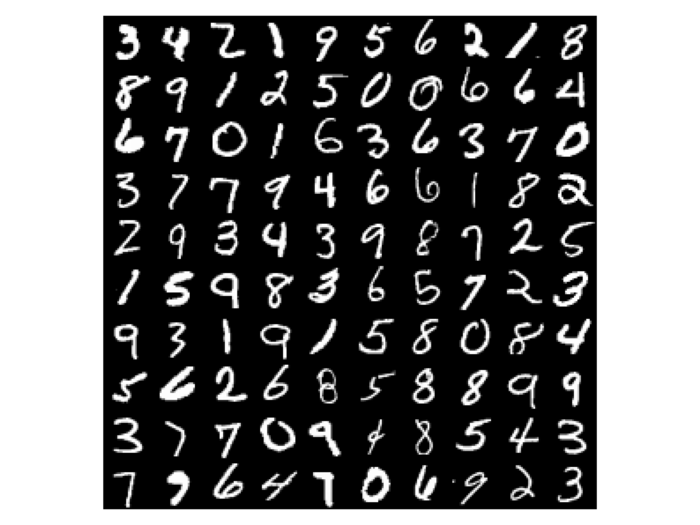
\includegraphics[width=7cm]{img/mnist-digits.png}
    \caption{Nasumično odabrani znakovi iz skupa MNIST}
    \label{fig:MNIST}
\end{figure}

Radi mogućnosti praćenja učenja te praćenja generalizacije mreže tijekom učenja potreban je jedan skup koji nije u skupu za učenje. Ispitni skup se ne može uzeti u obzir zato što on služi za konačno ispitivanje kvalitete mreže i ne smije se koristiti tijekom učenja, čak ni za praćenje pogreške jer može utjecati na konačne rezultate, tj. moglo bi se dogoditi da se podešavaju hiperparametre mreže tako da pogoduju baš tom skupu a da mreža ne generalizira općenito. Zato će se originalni skup za treniranje podijeliti u dva skupa, jedan za treniranje a drugi za validaciju. Skup za validaciju se neće koristiti za učenje ali će biti od koristi prilikom praćenja učenja i generalizacije mreže. Dakle prema novoj podjeli skup MNIST je podijeljen na:
\begin{itemize}
\item \textbf{skup za treniranje} - sadrži prvih 50 000 znakova originalnog skupa za treniranje
\item \textbf{skup za validaciju} - sadrži zadnjih 10 000 znakova originalnog skupa za treniranje
\item \textbf{skup za ispitivanje} - sadrži 10 000 znakova
\end{itemize}

\subsection{Predobrada ulaza}
Za uspješno učenje mreže, važno je da je aritmetička sredina skupa približno nula (da
bi učenje težina moglo krenuti u zahtijevanom smjeru) te da varijanca bude
približno jednaka jedan (da bi se zadržao opseg u sredini aktivacijske funkcije).
Za izvorni skup ne vrijedi ovo svojstvo. Stoga je svaki uzorak obrađen oduzimanjem 
aritmetičke sredine (samog uzorka) i normaliziranjem njegove varijance. Ujedno je i svakom uzorku dodan rub širine 2 te je time veličina ulaza proširena na dimenzije $32 \times 32$. Ova predobrada se mora raditi i na uzorcima iz skupa za testiranje.

\subsection{Minimalni skup za testiranje}
Prije nego što se započelo treniranje mreže na cijelom skupu za treniranje određen je minimalni skup za testiranje konvergencije mreže i ispravnosti implementacije. Taj skup se sastojao od svega 20 ulaza izdvojenih iz skupa MNIST te je sadržavao samo dvije klase (brojeve nule i jedinice). Mreža je prvo pokrenuta na ovom minimalnom skupu i kad je dobivena 100\%-tna točnost klasifikacije onda se tek počela trenirati na punom skupu.

\section{Odabrana arhitektura i hiperparametri mreže}
Odabrana je arhitektura slična arhitekturi \textit{LeNet} \citep{lecun1995convolutional} sa sljedećim slojevima:
\begin{itemize}
\item \textbf{Ulazni sloj} - jedna mapa veličine $32 \times 32$
\item \textbf{Prvi konvolucijski sloj} - 6 mapa veličine $28 \times 28$, 6 jezgri veličine $5 \times 5$
\item \textbf{Prvi aktivacijski sloj} - 6 mapa veličine $28 \times 28$
\item \textbf{Prvi sloj sažimanja} - 6 mapa veličine $14 \times 14$
\item \textbf{Drugi konvolucijski sloj} - 16 mapa veličine $10 \times 10$, 96 jezgri veličine $5 \times 5$
\item \textbf{Drugi aktivacijski sloj} - 16 mapa veličine $10 \times 10$
\item \textbf{Drugi sloj sažimanja} - 16 mapa veličine $5 \times 5$
\item \textbf{Treći konvolucijski sloj} - 100 mapa veličine $1 \times 1$, 1600 jezgri veličine $5 \times 5$
\item \textbf{Treći aktivacijski sloj} - 100 mapa veličine $28 \times 28$
\item \textbf{Prvi skriveni sloj} - 80 neurona
\item \textbf{Četvrti aktivacijski sloj} - 80 neurona
\item \textbf{Izlazni sloj} - drugi skriveni sloj s 10 neurona
\end{itemize}

Svi slojevi sažimanja imaju okvire veličine $2 \times 2$. Svi slojevi su potpuno povezani te se koristio stohastički gradijentni spust. Kao funkcija pogreške se koristila srednja kvadratna pogreška s time da se izlaz interpretirao kao vektor od 10 brojeva. Recimo očekivani izlaz za znamenku 7 bi bio $\{0,0,0,0,0,0,0,1,0,0\}$.

Mreža je trenirana sa 41 prolazom kroz skup za učenje sa stalnom stopom učenja $\eta=0.001$. Tijekom cijelog učenja se nakon svake epohe pratila prosječna pogreška te točnost klasifikacije na skupu za treniranje i validacijskom skupu. Na slici ~\ref{fig:graf-greska} se može vidjeti promjena prosječne pogreške tijekom učenja a na slici ~\ref{fig:graf-tocnost} promjena točnosti na skupu za treniranje i validacijskom skupu. Vidimo da su na oba grafa linije za validacijski skup i skup za treniranje jako blizu jedna drugoj. To znači da naučena mreža jako dobro generalizira te da nije došlo do prevelikog prilagođavanja skupu za učenje (engl. \textit{overfitting}).

\begin{figure}
    \centering
    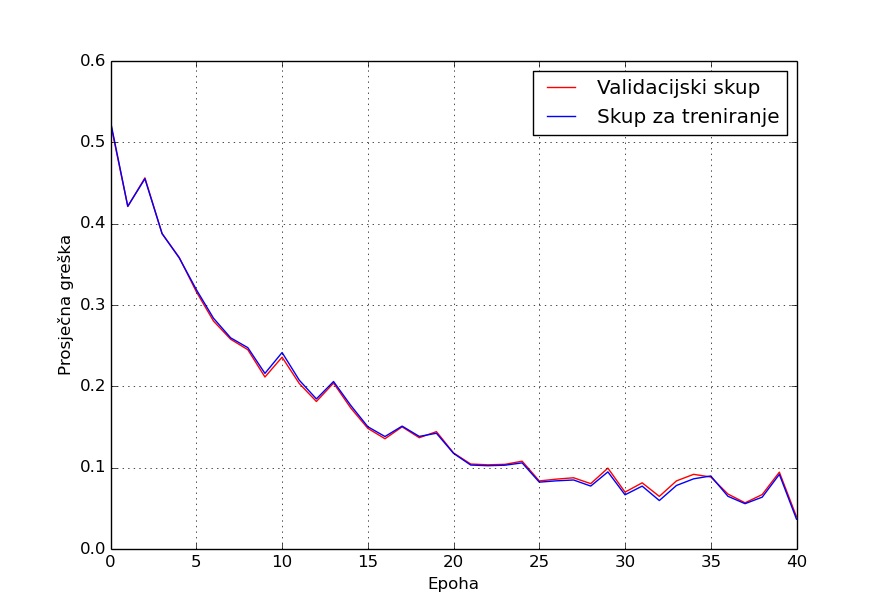
\includegraphics[width=14cm]{img/graf-greska.png}
    \caption{Promjena prosječne pogreške na validacijskom skupu i skupu za treniranje tijekom učenja}
    \label{fig:graf-greska}
\end{figure}

\begin{figure}
    \centering
    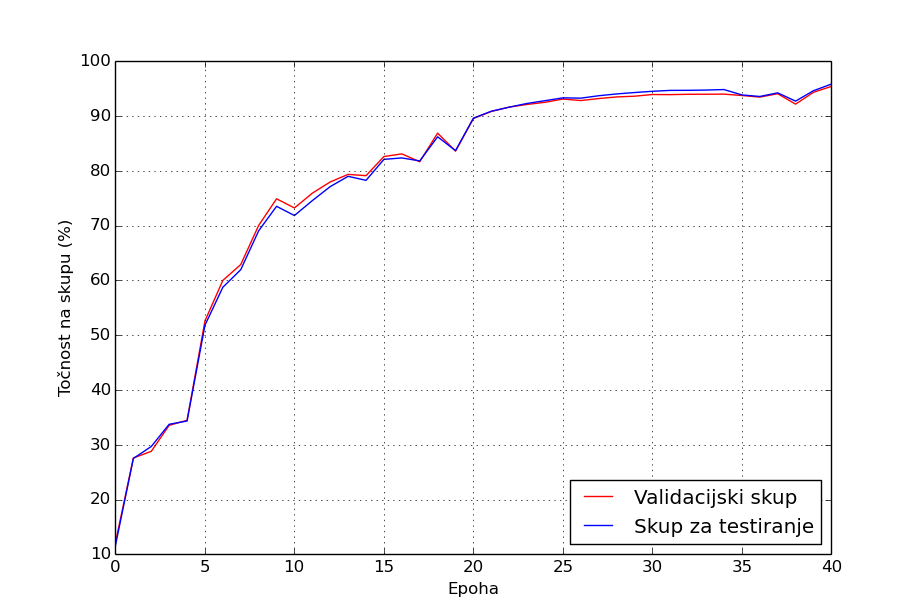
\includegraphics[width=14cm]{img/graf-tocnost.png}
    \caption{Promjena točnosti klasifikacije na validacijskom skupu i skupu za treniranje tijekom učenja}
    \label{fig:graf-tocnost}
\end{figure}

Ovako istrenirana mreža ima točnost (broj ispravno klasificiranih uzoraka) na ispitnom skupu od 95.21\%. Detaljni rezultati su dani matricom zabune u tablici ~\ref{tbl:matrica-zabune}.
 
\begin{table}
\caption{Matrica zabune}
\label{tbl:matrica-zabune}
\centering
\begin{tabular}{|c|c|c|c|c|c|c|c|c|c|c|c|} \hline
&\multicolumn{11}{|c|}{Predviđena klasa} \\ \hline
&&\textbf{0}&\textbf{1}&\textbf{2}&\textbf{3}&\textbf{4}&\textbf{5}&\textbf{6}&\textbf{7}&\textbf{8}&\textbf{9	}\\ \hline
\multirow{11}{*}{Stvarna klasa}
&\textbf{0}&966&0&1&0&0&0&2&0&3&8 \\
&\textbf{1}&0&1122&3&2&0&0&2&0&4&2 \\
&\textbf{2}&5&4&963&16&4&1&5&10&12&12 \\
&\textbf{3}&0&0&4&972&0&3&0&8&18&5 \\
&\textbf{4}&3&3&1&0&941&0&6&2&5&21 \\
&\textbf{5}&5&1&0&18&4&839&7&3&10&5 \\
&\textbf{6}&12&3&1&2&3&3&928&1&3&2 \\
&\textbf{7}&2&10&12&13&3&3&1&952&5&27 \\
&\textbf{8}&11&2&1&12&3&6&5&3&925&6 \\
&\textbf{9}&7&7&0&7&37&10&0&8&20&913 \\ \hline
\end{tabular}
\end{table}

Iz tablice možemo očitati najčešće greške, a to su:
\begin{itemize}
\item Broj 9 klasificiran kao broj 4 (37 krivih klasifikacija)
\item Broj 7 klasificiran kao broj 9 (27 krivih klasifikacija)
\item Broj 4 klasificiran kao broj 9 (21 krivih klasifikacija)
\item Broj 9 klasificiran kao broj 8 (20 krivih klasifikacija)
\end{itemize}

Vidljivo je da mreža ima najviše problema s klasifikacijom broja 9 zato što ga često klasificira kada su na ulazu drugi brojevi, a također ga često krivo klasificira (miješa ga sa 4, 7, i 8).

Svaki neuron u izlaznom sloju predstavlja jednu znamenku (ima ih 10). Kod određivanja znamenke odabire se neuron s najvećim izlazom. Ako se silazno sortiraju izlazi neurona u izlaznom sloju dobivaju se odabiri mreže prema prioritetu. Na primjer, ako je za dani ulaz izlaz petog neurona izlaznog sloja najveći mreža će taj ulaz klasificirati kao znamenku 5 te je ta znamenka najprioritetnija. Definirat ćemo rang pojedinog ulaza kao poziciju očekivane znamenke u listi prioriteta mreže. Za točno klasificirane ulaze je rang jednak 1, za ulaze kod kojih je točna klasa druga na listi prioriteta mreže je rang jednak 2 i tako dalje. U tablici ~\ref{tbl:rangovi} je prikazana frekvencija rangova za ispitni skup. Vidljivo je da velik broj krivo klasificiranih ulaza ima rang 2 (239) što znači da su točne klase za te ulaze bile drugi odabir mreže. Mali broj ulaza se nalazi i na lošijim rangovima što znači da su točne klase za te ulaze bile među zadnjim odabirima mreže.

\begin{table}
\caption{Frekvencija rangova za ispitni skup}
\label{tbl:rangovi}
\centering
\begin{tabular}{ll} \hline
Rang & Frekvencija \\ \hline
1 & 9521 \\
2 & 239 \\
3 & 78 \\
4 & 48 \\
5 & 28 \\
6 & 16 \\
7 & 22 \\
8 & 16 \\
9 & 21 \\
10 & 11 \\ \hline
\end{tabular}
\end{table}

Točnost mreže možemo prikazati i u ovisnosti o rangovima ulaza. To znači da će se za zadani rang svi ulazi koji imaju rang manji ili jednak zadanom smatrati točnima. U tablici ~\ref{tbl:tocnost-rangovi} je prikazana točnost mreže na ispitnom skupu u ovisnosti o rangovima ulaza. Vrijednosti u tablici se interpretiraju kao postotak ulaza za koje je rang manji ili jednak zadanome.

\begin{table}
\caption{Točnost mreže u ovisnosti o rangovima ulaza}
\label{tbl:tocnost-rangovi}
\centering
\begin{tabular}{ll} \hline
Rang & Točnost (\%) \\ \hline
1 & 95.21 \\
2 & 97.60 \\
3 & 98.38 \\
4 & 98.86 \\
5 & 99.14 \\
6 & 99.30 \\
7 & 99.52 \\
8 & 99.68 \\
9 & 99.89 \\
10 & 100.00 \\ \hline
\end{tabular}
\end{table}

\section{Usporedba rezultata sa drugim izvedbama}
U \citep{vukoticraspoznavanje} je napravljena slična konvolucijska neuronska mreža za testiranje na skupu MNIST. Mreža je poput ove napravljena bez korištenja vanjskih biblioteka za konvolucijske neuronske mreže. Takva izvedba je imala točnost od 98.67\% što je za 3.46\% bolje od mreže razvijene u ovom radu. Moguće objašnjenje ove razlike je korištenje posebnog skupa za validaciju koji je izdvojen iz skupa za učenje mreže zbog čega je mreža trenirana na manjem skupu. 

Mreža razvijena u ovom radu klasificira uzorke brzinom od 250 klasifikacija po sekundi što je značajno ubrzanje u odnosu na \citep{vukoticraspoznavanje} gdje jedna klasifikacija traje nekoliko sekundi.

\chapter{Zaključak}
Kroz ovaj rad je prikazan način rada dubokih neuronskih mreža s naglaskom na konvolucijske neuronske mreže. Proučene su specifičnosti konvolucijskih neuronskih mreža i razrađeni su detalji algoritma backpropagation. Također je razvijena implementacija konvolucijske neuronske mreže u programskom jeziku C++-u. Mreža je razvijena bez korištenja vanjskih biblioteka za konvolucijske neuronske mreže. 

Mreža je najprije zasebno testirana na minimalnom primjeru pomoću kojeg je provjereno ispravno funkcioniranje slojeva mreže, algoritma backpropagation i općenito svih ostalih dijelova implementacije. Nakon toga je mreža trenirana za klasifikaciju rukom pisanih znamenki iz skupa MNIST. Cijeli proces učenja mreže je pomno praćen i analiziran. Iz analize učenja mreže je zaključeno da je generalizacija mreže vrhunska jer je razlika između klasifikacije na skupu za učenje i validacijskom skupu minimalna kroz cijeli proces učenja. S takvom mrežom je postignut rezultat od 95.21\% ispravno klasificiranih uzoraka na skupu za ispitivanje. Ako uzmemo u obzir da su se s konvolucijskim neuronskim mrežama postizale točnosti i preko 98\% za skup MNIST, ovaj rezultat, iako izvrstan, je malo ispod očekivanja za konvolucijsku neuronsku mrežu. Moguće objašnjenje ovog rezultata je to što nismo koristili cijeli skup za učenje tijekom treniranja mreže. U daljnjem radu se preporučuje treniranje mreže na cijelom skupu za učenje radi poboljšanja točnosti mreže.

Pošto je ovaj rad izrađen za primjenu na osobnim računalima opće namjene cijeli program se izvodio na jednoj jezgri CPU-a. Brzina programa je iznenađujuće dobra s čak i preko 250 klasifikacija u sekundi što je i više nego zadovoljavajuće za primjenu na računalima opće namjene. Ako je potrebna još veća brzina u daljnjem radu se program može paralelizirati.

Pošto u ovom radu nije bilo dovoljno vremena za optimizaciju svih hiperparametara u daljnjem radu se preporučuje testiranje mreže s drugačijom arhitekturom, aktivacijskim funkcijama i funkcijama pogreške. Također se preporučuje razvijanje dodatnih metoda koje pospješuju učenje i konvergenciju mreže poput metode slučajnog izostavljanja neurona prilikom učenja (engl. \textit{dropout}) i dodavanja inercije.


\bibliography{literatura}
\bibliographystyle{fer}

\begin{sazetak}
U ovom radu je prikazan način rada dubokih neuronskih mreža sa naglaskom na konvolucijske mreže. Razvijena je implementacija konvolucijske neuronske mreže za računala opće namjene i opisan je postupak učenja mreže algoritmom backpropagation. Mreža je trenirana i vrednovana na skupu rukom pisanih znamenki MNIST. Na kraju su prikazani i opisani dobiveni rezultati te su analizirane karakteristike i učinak naučene mreže.

\kljucnerijeci{umjetne neuronske mreže, duboke neuronske mreže, konvolucijske neuronske mreže, klasifikacija, gradijentni spust, strojno učenje, računalni vid, raspoznavanje objekata}
\end{sazetak}

% TODO: Navedite naslov na engleskom jeziku.
\engtitle{Object recognition with convolutional neural networks}
\begin{abstract}
In this work an overview of deep neural networks was made with emphasis on convolutional neural networks. Program implementation of convolutional neural network was developed for general purpose computers. Learning algorithm backpropagation was explained and developed. The network was trained and evaluated on the MNIST database of handwritten digits. In the end evaluation results were shown and networks characteristics and performance was analyzed.

\keywords{artificial neural networks, deep neural networks, convolutional neural networks, classification, gradient descent, machine learning, computer vision, object recognition}
\end{abstract}

\end{document}
